\subsection{Fase di progettazione architetturale}
\subsubsection{Prospetto orario}
In questa fase, la distribuzione oraria dei componenti del gruppo è la seguente:

{

\rowcolors{2}{azzurro2}{azzurro3}

\centering
\renewcommand{\arraystretch}{1.8}
\begin{longtable}{C{4cm} C{1cm} C{1cm} C{1cm} C{1cm} C{1cm} C{1cm} C{2cm}}

\rowcolor{azzurro1}
\textbf{Nominativo} &
\textbf{RE}&
\textbf{AM}&
\textbf{AN}&
\textbf{PT}&
\textbf{PR}&
\textbf{VE}&
\textbf{Ore totali}\\
\endhead

\MB & 0 & 8 & 0 & 12 & 4 & 8 & 32 \\
\VAS & 6 & 0 & 10 & 4 & 4 & 8 & 32 \\
\FD & 0 & 10 & 7 & 8 & 0 & 7 & 32 \\
\NM & 10 & 0 & 6 & 8 & 0 & 8 & 32 \\
\SB & 0 & 0 & 5 & 12 & 5 & 10 & 32 \\
\GB & 0 & 6 & 0 & 10 & 6 & 10 & 32 \\
\MDI & 0 & 4 & 0 & 12 & 5 & 11 & 32 \\
\textbf{Ore Totali} & 16 & 28 & 28 & 66 & 24 & 62 & 224 \\

\rowcolor{white}
\caption{Distribuzione oraria nel periodo di progettazione architetturale}\\

\end{longtable}
}
\newpage
Il seguente istogramma riassume i dati ottenuti:

\begin{figure}[H]
\centering
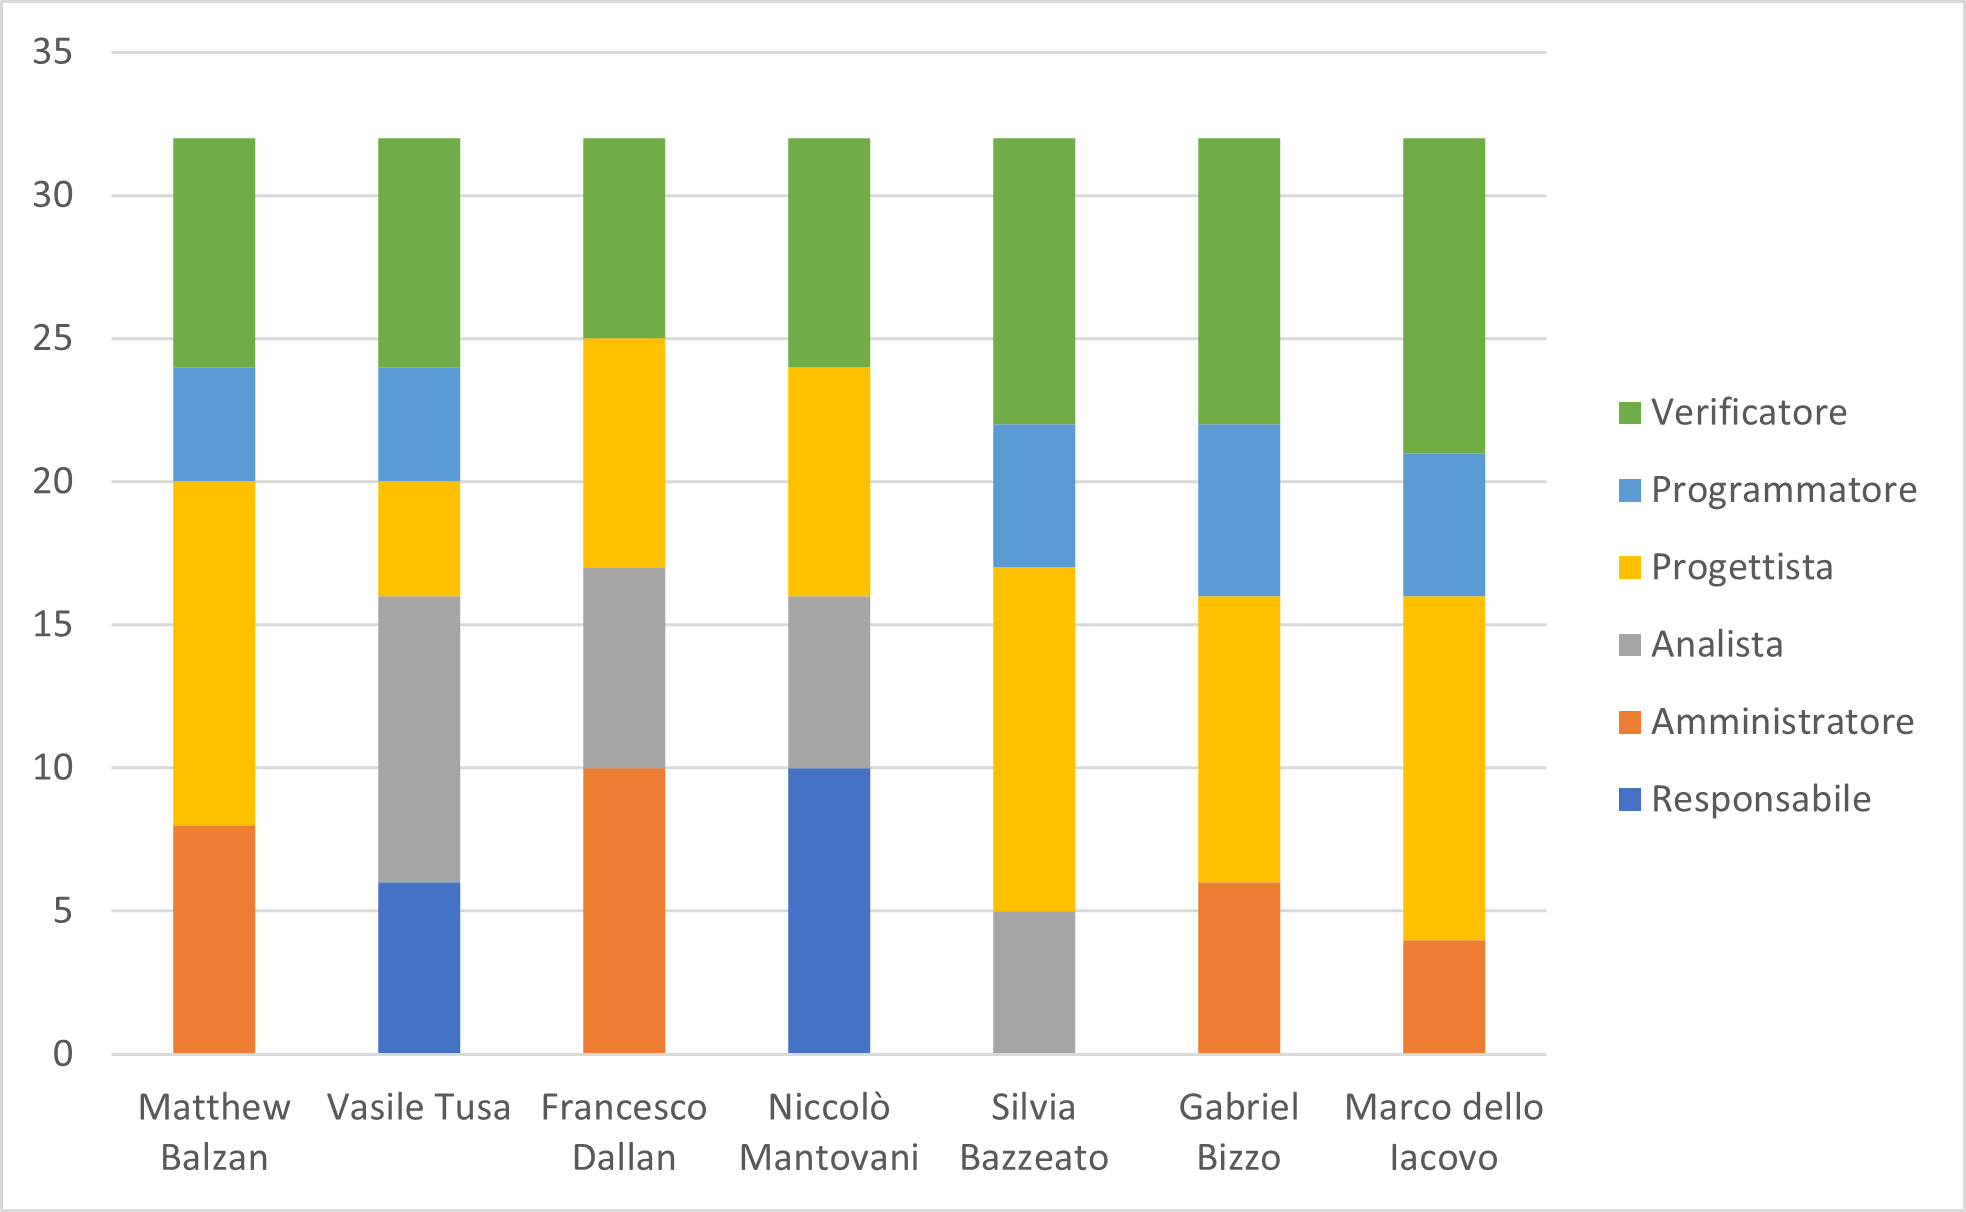
\includegraphics[scale=0.90]{res/Preventivo/Img/istogramma_progettazione}\\
\caption{Istogramma della ripartizione dei ruoli nel periodo di progettazione architetturale}
\end{figure}


\subsubsection{Prospetto economico}

In questa fase, il costo per ogni ruolo è il seguente:

{

\rowcolors{2}{azzurro2}{azzurro3}

\centering
\renewcommand{\arraystretch}{1.8}
\begin{longtable}{C{3cm} C{1cm} C{2cm} }

\rowcolor{azzurro1}
\textbf{Ruolo} &
\textbf{Ore}&
\textbf{Costo}\\
\endhead

\textit{Responsabile} & 16 & 480\euro{} \\
\ammProg & 28 & 560\euro{} \\
\analProg & 28 & 700\euro{} \\
\progetProg & 66 & 1452\euro{} \\
\programProg & 24 & 360\euro{} \\
\verifProg & 62 & 930\euro{} \\
\textbf{Totale} & 224 & 4482\euro{} \\

\rowcolor{white}
\caption{Prospetto dei costi per ruolo nel periodo di progettazione architetturale}\\

\end{longtable}
}
\newpage
Il seguente areogramma riassume i dati ottenuti:

\begin{figure}[H]
\centering
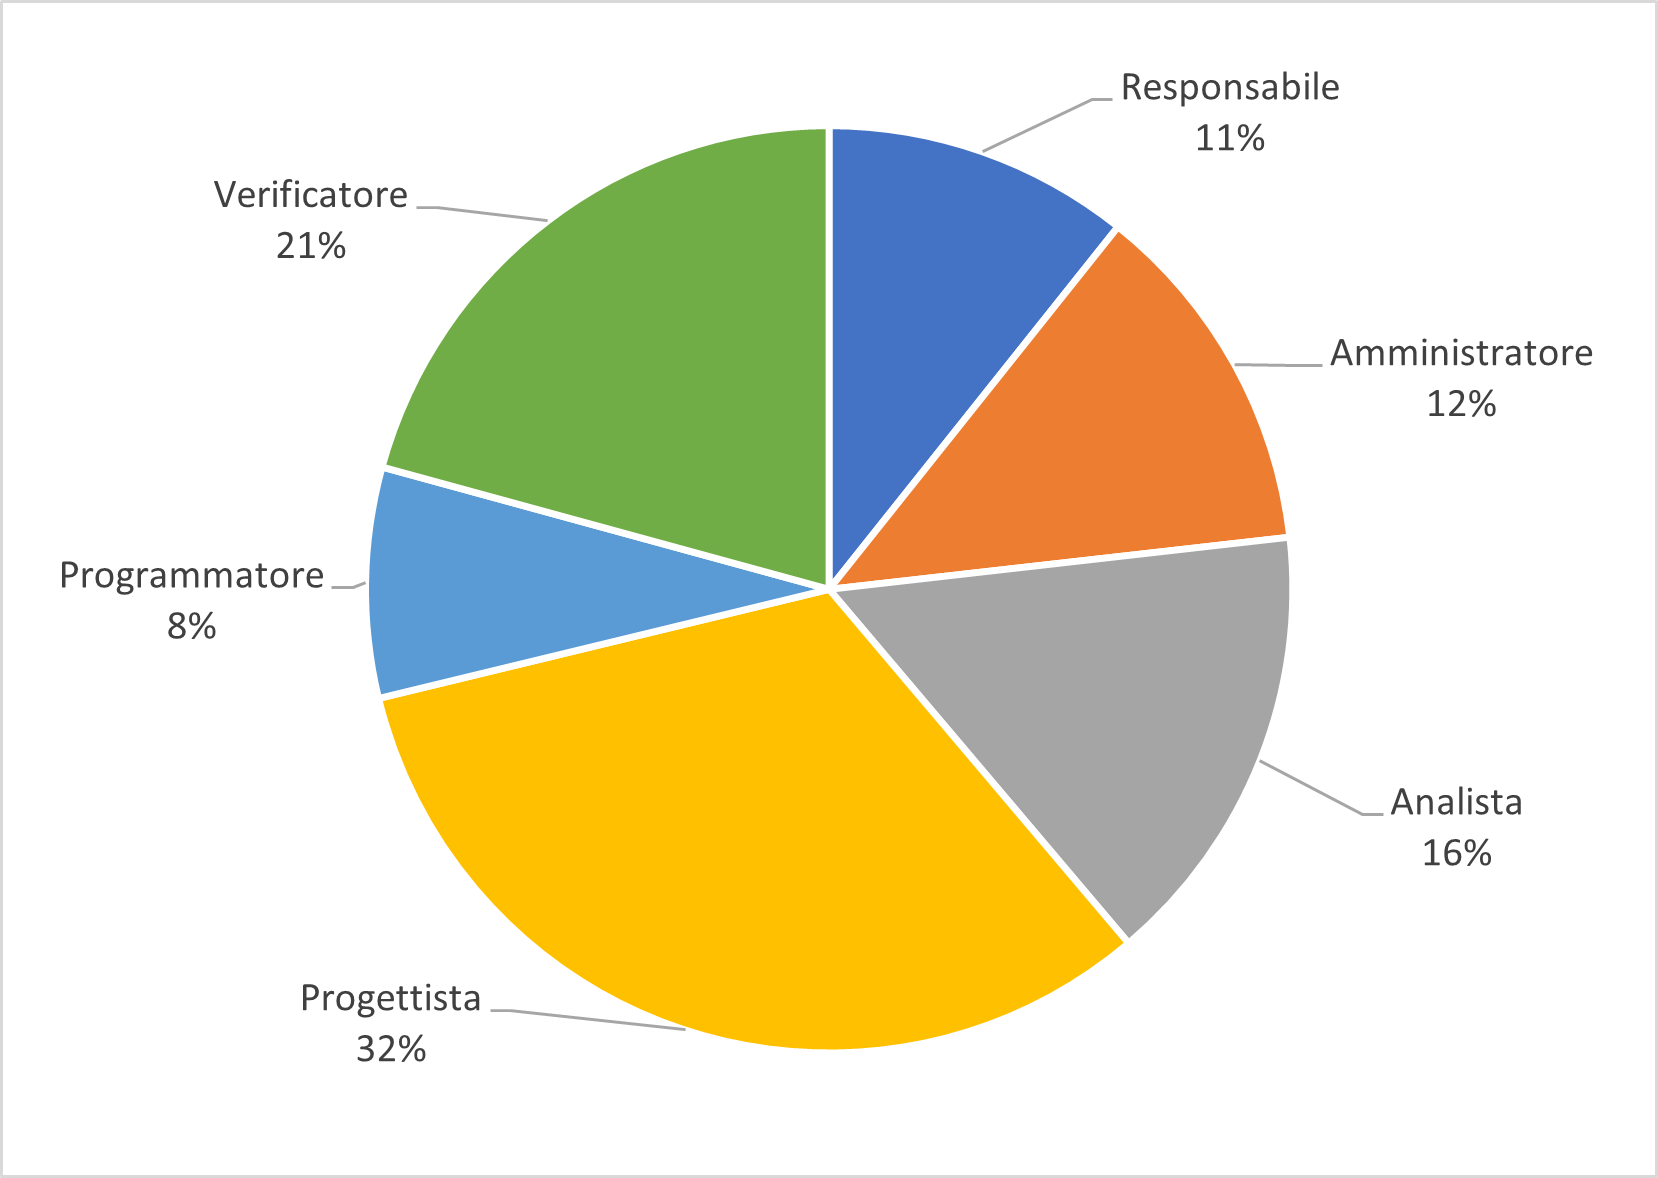
\includegraphics[scale=0.90]{res/Preventivo/Img/areogramma_progettazione}\\
\caption{Areogramma della distribuzione economica nel periodo di progettazione architetturale}
\end{figure}





